%% LyX 2.1.3 created this file.  For more info, see http://www.lyx.org/.
%% Do not edit unless you really know what you are doing.
\documentclass[russian,english]{beamer}
\usepackage[T2A,OT2,T1]{fontenc}
\usepackage[utf8x]{inputenc}
\setcounter{secnumdepth}{3}
\setcounter{tocdepth}{3}
\usepackage{babel}
\usepackage{graphicx}
\ifx\hypersetup\undefined
  \AtBeginDocument{%
    \hypersetup{unicode=true,
 bookmarks=true,bookmarksnumbered=true,bookmarksopen=false,
 breaklinks=false,pdfborder={0 0 1},backref=false,colorlinks=true,pdftitle={Reviving the Old Russian orthography for the 21st century},
 pdfauthor={Sergei Winitzki},
 pdfsubject={computer word processing},
 linkcolor=black,urlcolor=blue}
  }
\else
  \hypersetup{unicode=true,
 bookmarks=true,bookmarksnumbered=true,bookmarksopen=false,
 breaklinks=false,pdfborder={0 0 1},backref=false,colorlinks=true,pdftitle={Reviving the Old Russian orthography for the 21st century},
 pdfauthor={Sergei Winitzki},
 pdfsubject={computer word processing},
 linkcolor=black,urlcolor=blue}
\fi
\usepackage{breakurl}

\makeatletter

%%%%%%%%%%%%%%%%%%%%%%%%%%%%%% LyX specific LaTeX commands.
\DeclareRobustCommand{\cyrtext}{%
  \fontencoding{T2A}\selectfont\def\encodingdefault{T2A}}
\DeclareRobustCommand{\textcyr}[1]{\leavevmode{\cyrtext #1}}
\AtBeginDocument{\DeclareFontEncoding{T2A}{}{}}


%%%%%%%%%%%%%%%%%%%%%%%%%%%%%% Textclass specific LaTeX commands.
 % this default might be overridden by plain title style
 \newcommand\makebeamertitle{\frame{\maketitle}}%
 % (ERT) argument for the TOC
 \AtBeginDocument{%
   \let\origtableofcontents=\tableofcontents
   \def\tableofcontents{\@ifnextchar[{\origtableofcontents}{\gobbletableofcontents}}
   \def\gobbletableofcontents#1{\origtableofcontents}
 }

%%%%%%%%%%%%%%%%%%%%%%%%%%%%%% User specified LaTeX commands.
\usetheme[secheader]{Boadilla}
\usecolortheme{seahorse}
\title[Old Russian Orthography]{Reviving the Traditional Russian Orthography for the 21st Century}
\author{Sergei Winitzki}
\date{April 24, 2015}
\institute[Versal Group Inc.]{Text By The Bay 2015}

\makeatother

\begin{document}
\frame{\titlepage}
\begin{frame}{Old Russian Orthography\texttt{: what and why}}

\begin{itemize}
\item The Russian orthography was reformed in 1918

\begin{itemize}
\item 4 letters \foreignlanguage{russian}{Ѣѣ, Ѳѳ, Іі, Ѵѵ} were physically
removed from printing presses

\begin{itemize}
\item Often, \foreignlanguage{russian}{Ъъ} was also removed by mistake
\end{itemize}
\end{itemize}
\item Classic Russian literature used the old orthography:

\begin{itemize}
\item Pushkin, Turgenev, Dostoyevsky, Tolstoy, Chekhov, Nabokov, ...
\end{itemize}
\end{itemize}
\end{frame}

\begin{frame}{Old English orthography: example}


Hobbes, \emph{De cive} (1651)

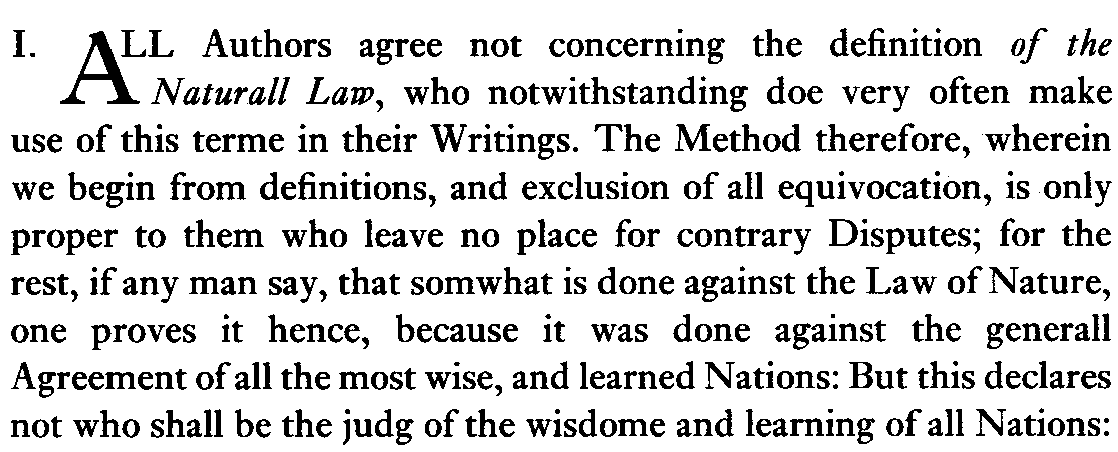
\includegraphics[width=1\textwidth]{Hobbes_-_De_Cive_-_1651}
\end{frame}

\begin{frame}{Old Russian orthography: example}


Nabokov, \emph{Storm} (1930)

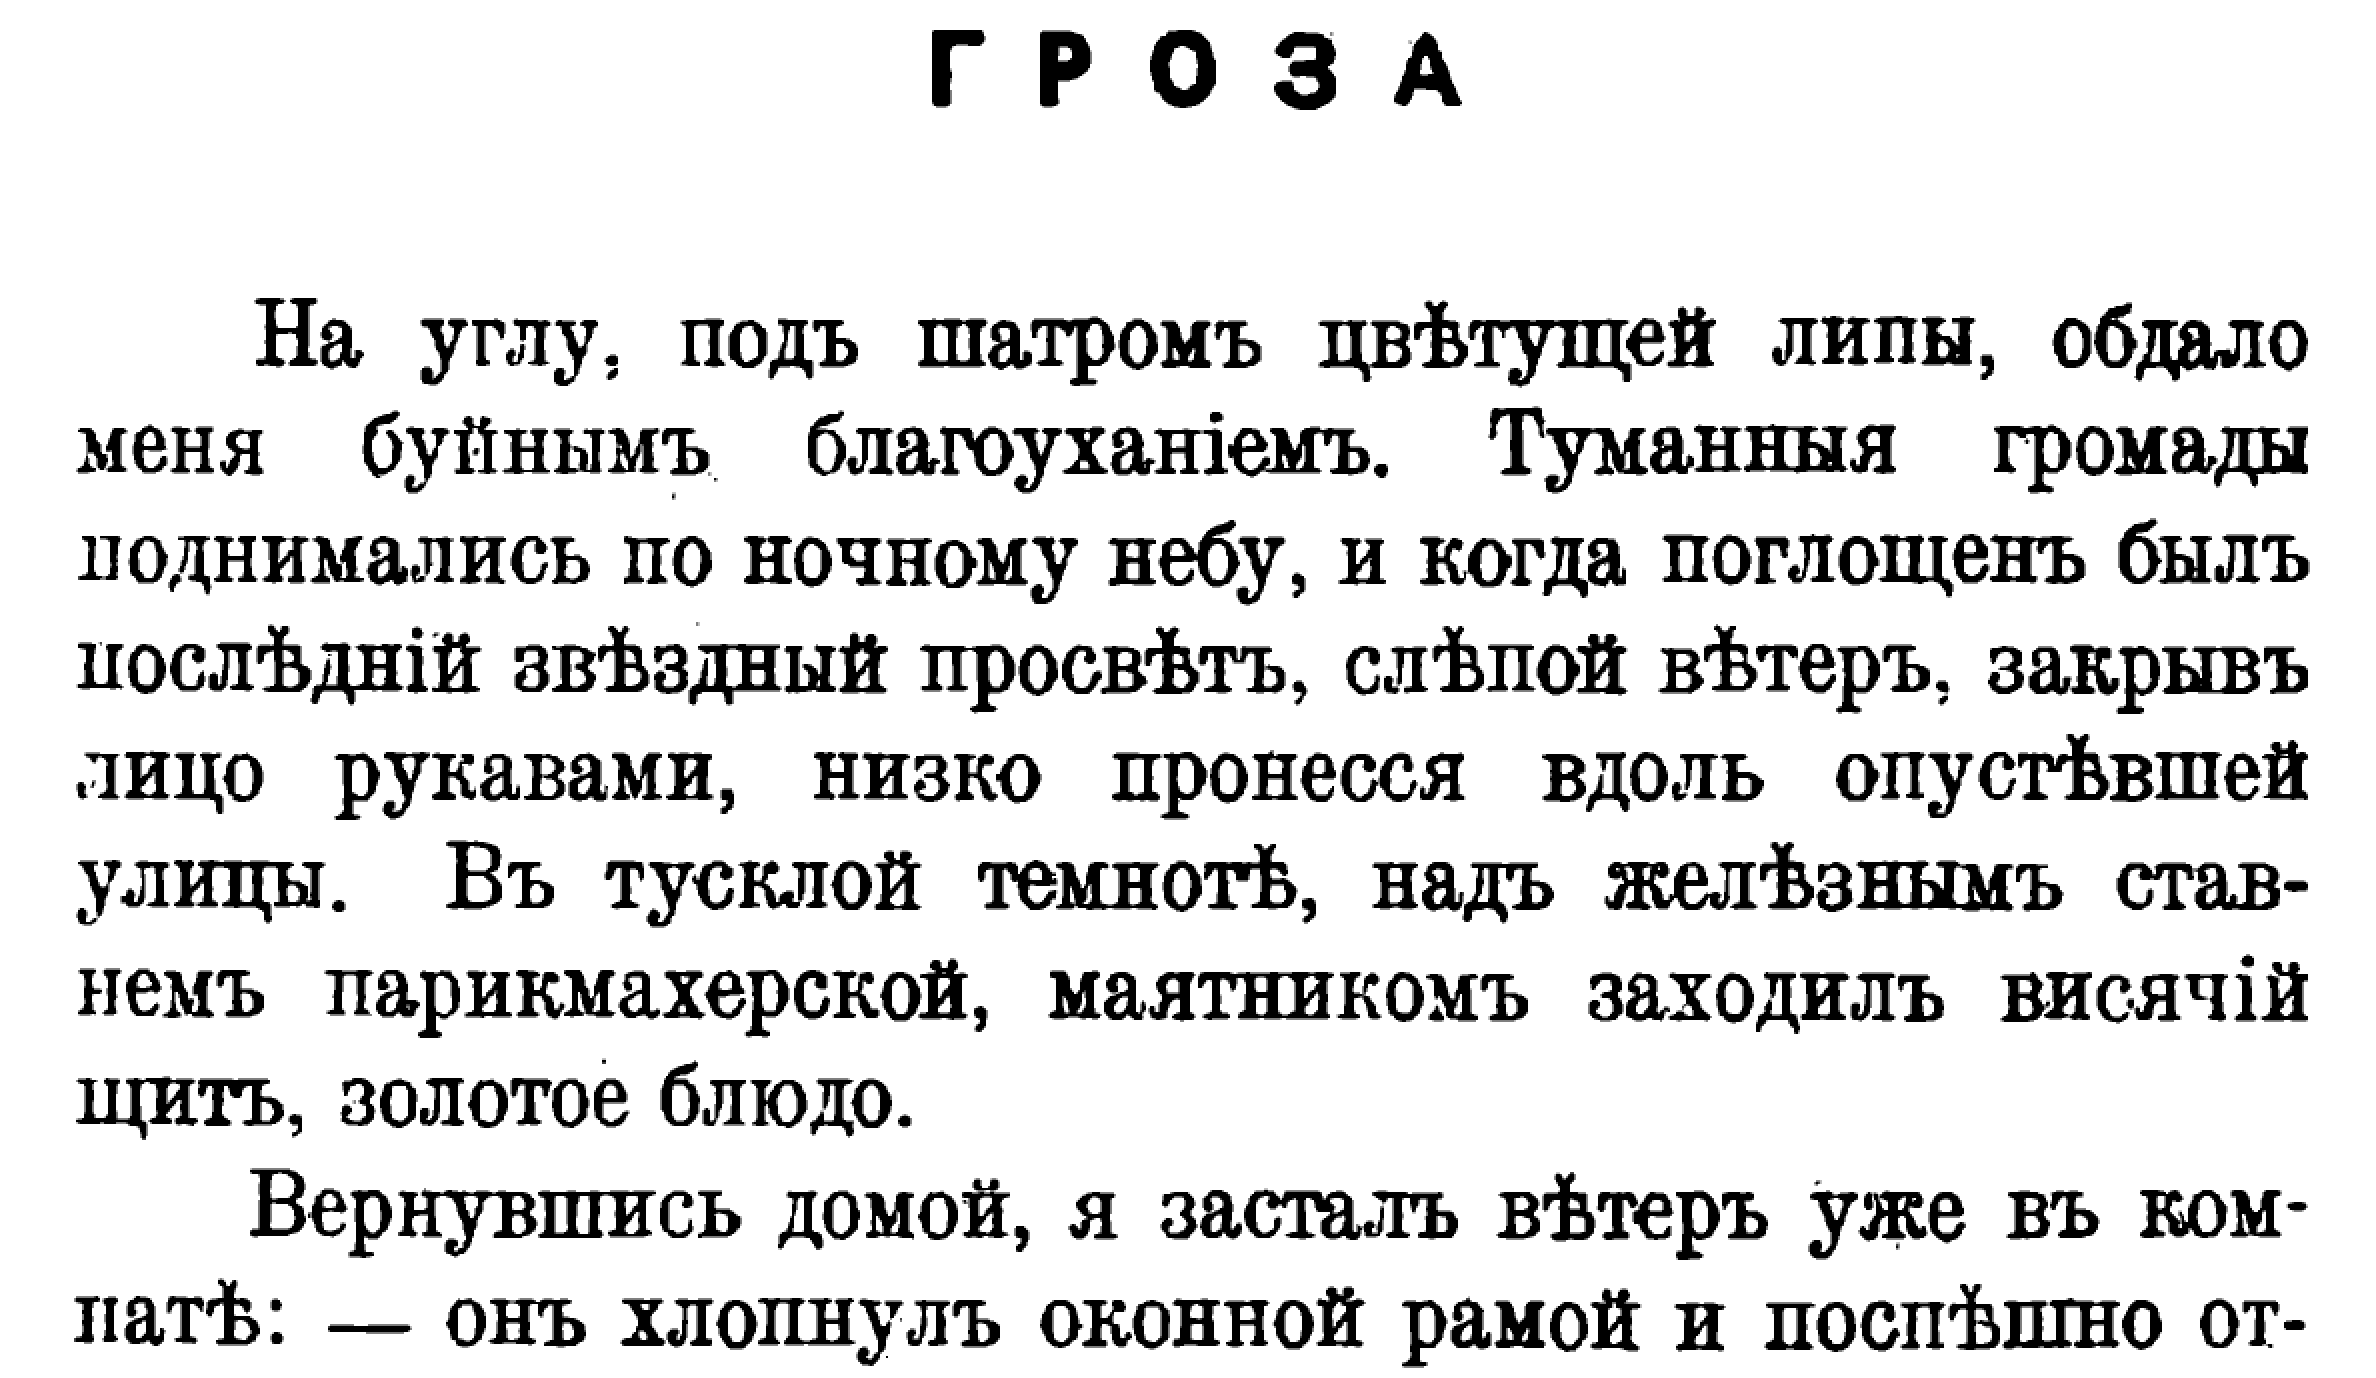
\includegraphics[width=1\textwidth]{Sirin_-_Groza_1930}
\end{frame}

\begin{frame}{Main challenges in processing old Russian orthography}

\begin{itemize}
\item As of 2000, no 8-bit encodings contained the letters \foreignlanguage{russian}{Ѣѣ,
Ѳѳ, Іі, Ѵѵ} 

\begin{itemize}
\item Unicode support was not widespread
\end{itemize}
\item No keyboard layouts, no screen fonts, few vector fonts 

\begin{itemize}
\item \LaTeX{} font support: nonstandard font encoding by AMS
\end{itemize}
\item No spelling checker support, no OCR, no hyphenation
\end{itemize}
\end{frame}

\begin{frame}{State of the art in 2015}

\begin{itemize}
\item The letters \foreignlanguage{russian}{Ѣѣ, Ѳѳ, Іі, Ѵѵ} are present
in most Cyrillic fonts 

\begin{itemize}
\item typesetting, printing supported through Unicode
\item \LaTeX{} font support: OT2 font encoding only!
\end{itemize}
\item Some spelling checker support (ispell, AbiWord, Open Office)
\item Some language support for OCR
\item No hyphenation support, no standard keyboard layouts
\end{itemize}
\end{frame}

\begin{frame}{The KOI8-C project (1999-2003)}

\begin{itemize}
\item \href{http://oldrus-ispell.sourceforge.net}{http://oldrus-ispell.sourceforge.net}
\item KOI8-C encoding (\href{http://www.ietf.org/archive/id/draft-winitzki-koi8c-encoding-00.txt}{IETF draft})
\item Bitmapped X-Window fonts (BDF), the \texttt{xcyr} package

\begin{itemize}
\item Became part of \texttt{\href{http://www.cl.cam.ac.uk/~mgk25/ucs-fonts.html}{ucs-fonts}}
and \texttt{\href{https://packages.debian.org/sid/xfonts-cyrillic}{xfonts-cyrillic}}
\end{itemize}
\item \texttt{ispell} dictionary for old Russian orthography
\item PostScript typesetter using BDF as Type 3 fonts
\item A primitive converter from new to old orthography
\end{itemize}
\end{frame}

\begin{frame}{The KOI8-C encoding and screen fonts}


Viewing Nabokov, \emph{Despair} (1934) in Netscape using KO8-C

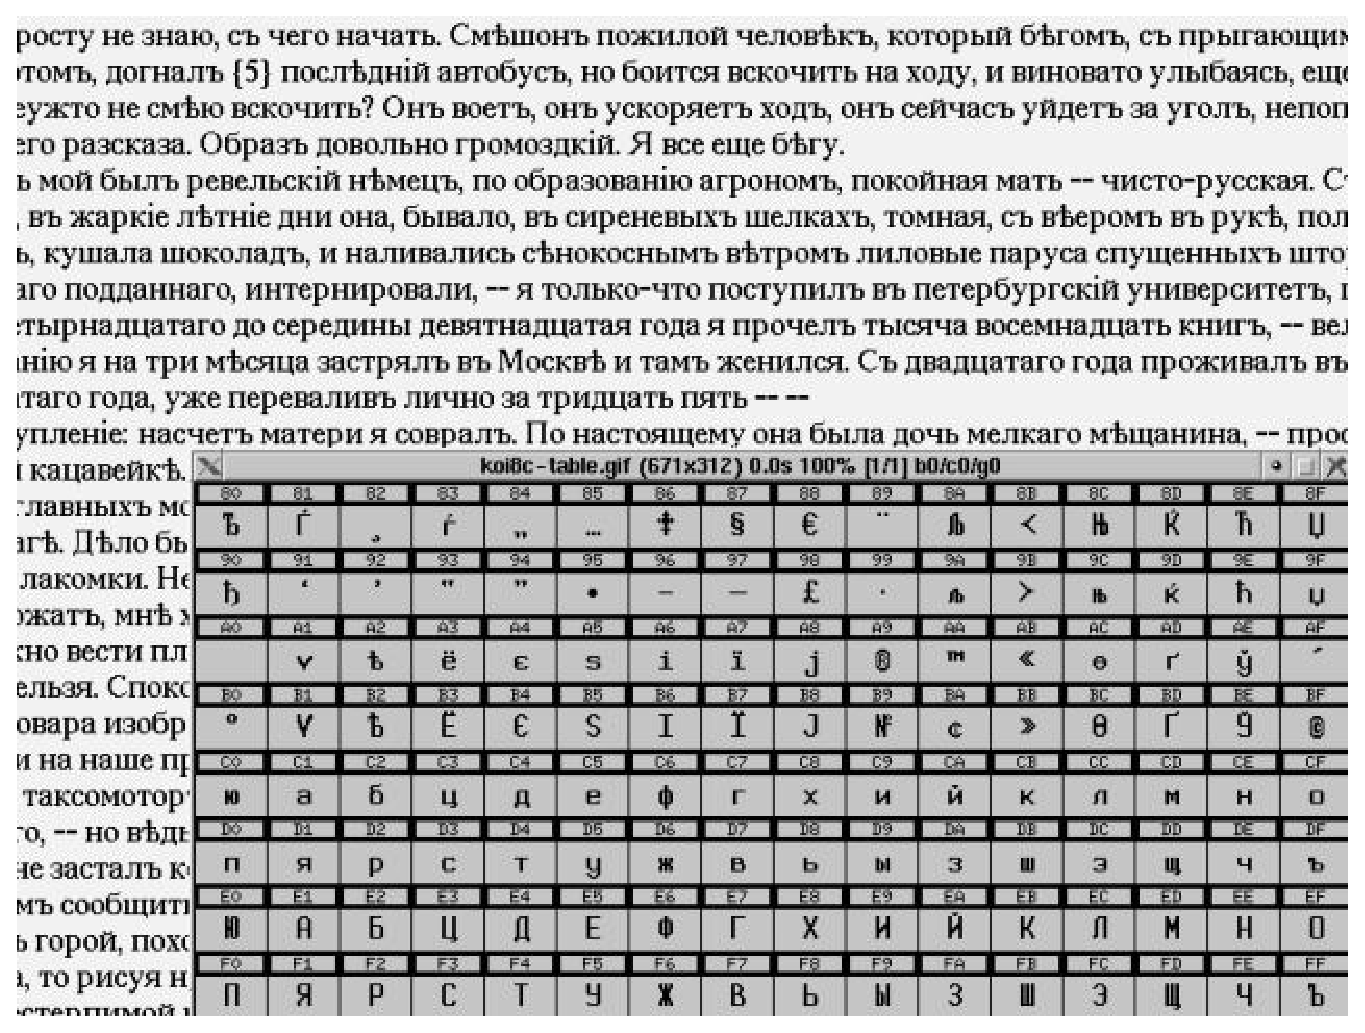
\includegraphics[height=0.8\textheight]{xcyr-screenshot}
\end{frame}

\begin{frame}{Working with the oldrus-ispell dictionary}


Proofreading Melgunov's ``Red Terror in Russia'' (1924)

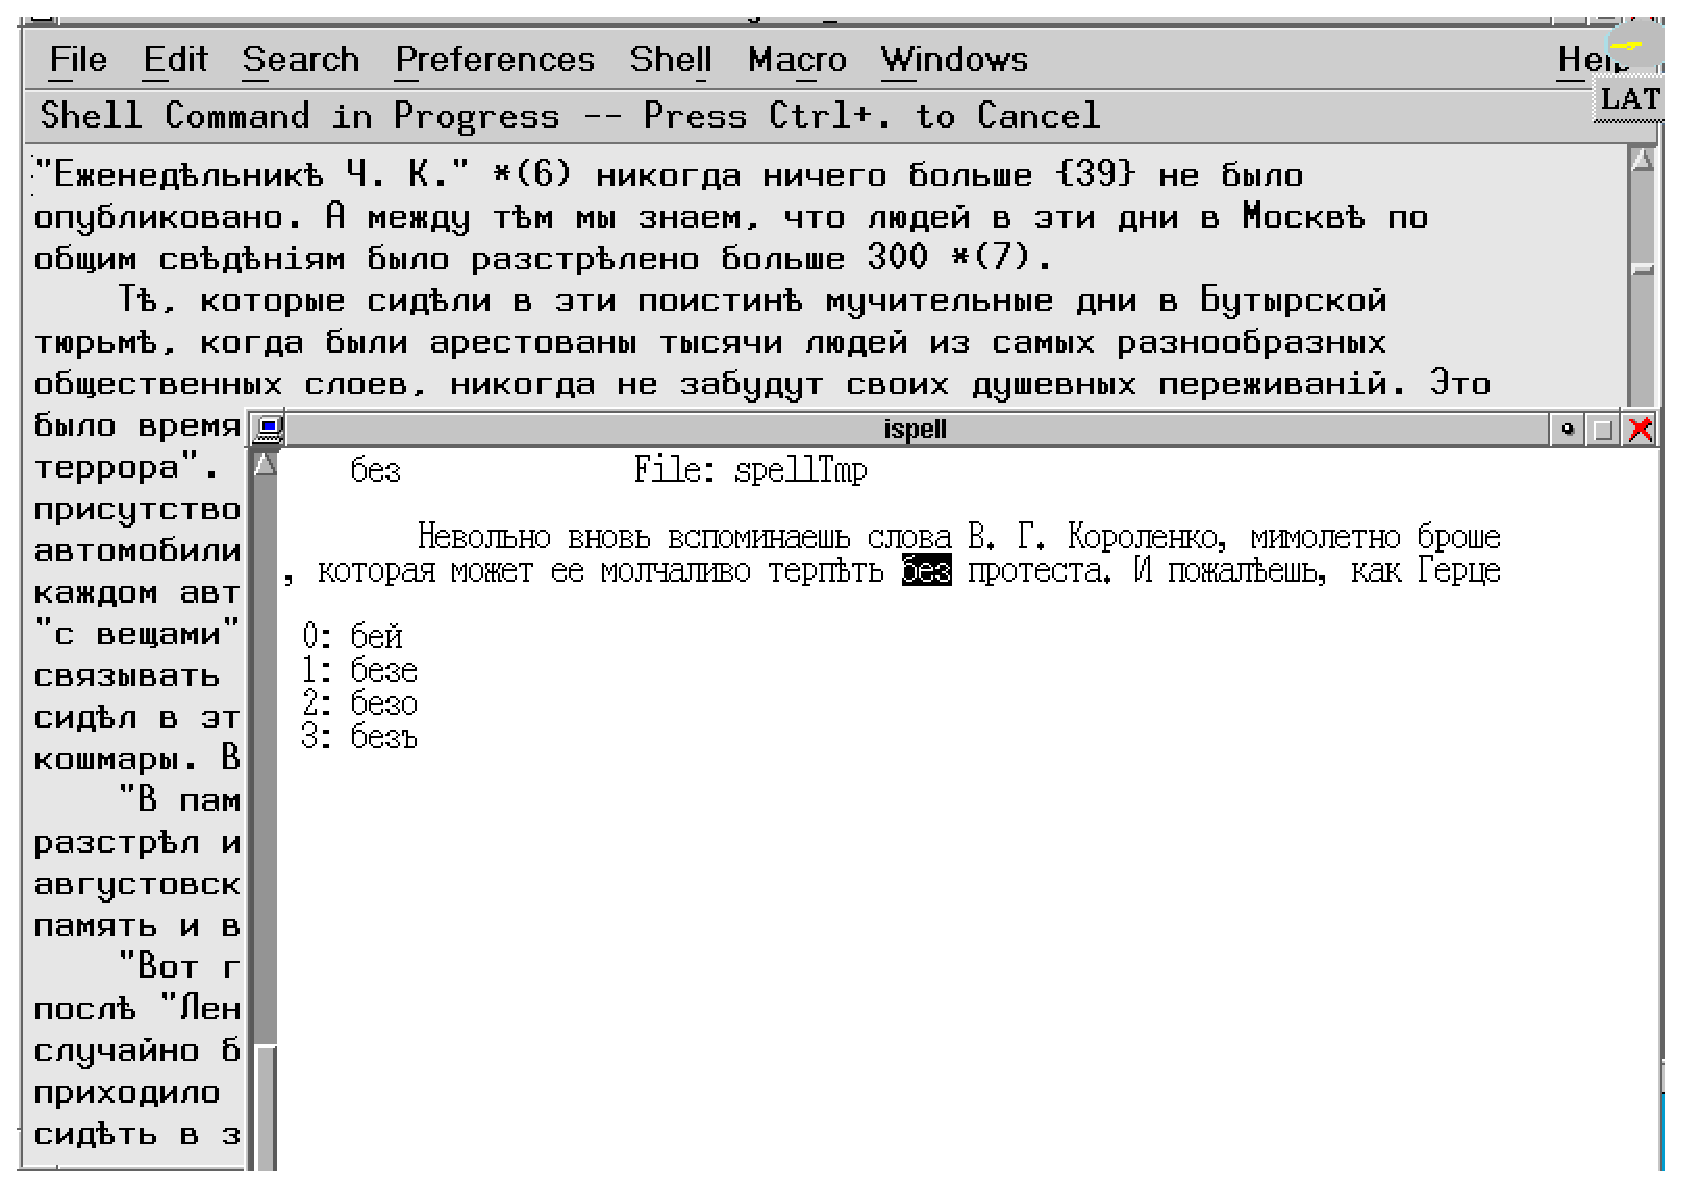
\includegraphics[width=1.2\textwidth]{oldrus-screenshot}
\end{frame}

\begin{frame}{Main challenges}

\end{frame}

\begin{frame}{Main challenges}

\end{frame}

\begin{frame}{Main challenges}
\end{frame}

\end{document}
